\documentclass[12pt]{article}
\usepackage{amsmath,amsthm,amsfonts,amssymb,epsfig,graphicx,subcaption,placeins}


\bibliographystyle{plain}

\textheight 24cm
\textwidth 15cm
\topmargin -3cm
\oddsidemargin -0.1cm
\evensidemargin 5cm

\newcommand{\reals}{\mathbb{R}}
\newcommand{\naturals}{\mathbb{N}}
\newcommand{\complex}{\mathbb{C}}
\newcommand{\integers}{\mathbb{Z}}
\newcommand{\banach}{\mathbb{B}}
\newcommand{\exponent}{\operatorname{e}}
\newcommand{\diag}{\operatorname{diag}}
\newcommand{\interior}{\operatorname{int}}
\newcommand{\deter}{\operatorname{det}}



%\theoremstyle{plain}
%\newtheorem{defi}{Definition}
%\newtheorem{prop}{Proposition}
\newtheorem{stel}{Theorem}
\newtheorem{gevolg}{Corollary}
\newtheorem{lemma}{Lemma}
\theoremstyle{remark}
\newtheorem{opm}{Remark}

\begin{document}

\title{Division of labor in socially structured populations}

\author{Bryan K. Lynn\footnote{Department of Integrative Biology, Oregon State University, lynnbry@oregonstate.edu} and Patrick De Leenheer\footnote{Department of Mathematics and Department of Integrative Biology, Oregon State University, Supported in part by NSF-DMS-1411853, deleenhp@math.oregonstate.edu}}

\date{}

\maketitle


\begin{abstract}
Cooperating behaviors abound across all domains of life, but are vulnerable to invasion by cheaters. An important evolutionary question is to determine mechanisms that stabilize and maintain cooperation levels and prevent population collapse. Policing is one strategy populations may employ to achieve this goal, and it has been observed in many natural populations including microbes. 
Here we present and analyze a division of labor model to support that policing can indeed be a cooperation-stabilizing mediator.
\end{abstract}




\section{Introduction}

Acts of cooperation are found in a wide variety of species, ranging from bacteria to animals. Many bacteria cooperate by secreting extracellular products, so-called ``public goods", such as  biosurfactants for swarming \cite{xavier}, extracellular proteases to access food sources \cite{finkelstein}, and  siderophores for the purpose of iron-scavenging \cite{harrison}. Many higher organisms, including our own, have developed diversely structured societies where individuals take on specific roles to provide goods or services to the benefit of the population.

Despite the ubiquity of cooperation across all domains of life, populations are vulnerable to invasion by non-cooperating cheaters, including in several microbial systems \cite{velicer2,greig,ennis}. Indeed, cheaters that do not invest in cooperation do not incur a fitness cost, and are expected to exhibit a growth advantage compared to cooperators, at least initially. In the long run however, decreased cooperation levels can lead to the collapse of the population, a phenomenon commonly known as the Tragedy of the Commons 
\cite{hardin,tragedy,MBE}. This brings up the important but difficult evolutionary problem to identify mechanisms that maintain cooperative behaviors  \cite{hamilton,sachs}.


Various control mechanisms have been proposed that either coerce individuals into cooperating or constrain them from cheating \cite{foster,ratnieks,schuster,travisano}. One such mechanism is policing, which has been found across biological scales in nature \cite{cheating-wikipedia} such as in humans, rhesus monkeys, eusocial insects \cite{ratnieks2007,wenseleers,wenseleers-bees} like ants, bees and wasps (where egg-laying workers are treated aggressively, or have their eggs eaten) and even in symbiotic partnerships like cleaner and cleaning fish, and in nitrogen-fixating rhizobium and plants. Policing strategies have also developed in bacterial populations, as confirmed in experimental work in \cite{wang,manhes,smalley}. In \cite{wang} for example, it is shown that cooperators in {\it Pseudomonas aeruginosa} can secrete toxins such as cyanide, affecting cheaters but not the toxin-producers because they also activate detoxification genes when producing toxins. 

In this paper we propose a conceptual division-of-labor model to investigate if and how policing strategies can stabilize cooperative behavior. 
The model tracks 3 strains -cooperator, toxin-producer and cheater-, externally supplied growth nutrient, the public good produced by the cooperator that is required for growth, 
and the toxin that harms cooperators and cheaters. We find that when challenged by cheaters, cooperative behavior can indeed be stabilized, provided that the following conditions hold: 
\begin{enumerate}
\item Toxin-producers must be present. 
\item The cost of toxin production must exceed the cost of public good production. In other words, policing is more expensive than cooperation. 
\item The harmful effects of the toxin on the cooperator must be sufficiently high. This is a trade-off to offset that policing is more expensive than cooperation.
\item The effects of the toxin on the cheater must be even higher.
\end{enumerate}
These 4 items will be made precise in terms of various parameters and functional forms in the model.



\section{A division of labor chemostat model}

We consider a general chemostat model with positive dilution rate
$D$ and positive input nutrient concentration $S^0$. There are 3 microbial species, the cooperators, toxin producers, and the cheaters whose concentrations are denoted as 
$X_1$, $X_2$ and $X_3$ respectively. The nutrient concentration in the chemostat has concentration $S$. 
The cooperator produces a public good with concentration $E$, which is required for growth of all 3 species. Public goods in microbial populations are typically enzymes that facilitate nutrient uptake. The toxin producers produce a toxin with concentration $T$, and the positive toxicity rate constant for cooperators and cheaters is $K_1$ and $K_3$ respectively. Toxin producers are resistant to the toxin they produce. Thus, cooperators and toxin producers have specialized tasks, leading to a division-of-labor model below.


Nutrient is consumed by each of the species at per capita rate $F(S,E)/\gamma_i$, for $i=1,2,3$, where $\gamma_i$ is the yield in the conversion of nutrient into new biomass of species $X_i$. We assume that  $F(S,E)$ is non-negative and twice continuously differentiable for all $S\geq 0$ and $E\geq 0$, and satisfies the following assumptions:
\begin{eqnarray*}
{\bf H1}:&& F(0,E)=F(S,0)=0,\\
&& F(S,E)>0 \textrm{ when } S>0 \textrm{ and }E>0,\\
&&\frac{\partial F}{\partial S}(S,E)>0 \textrm{ and } \frac{\partial F}{\partial E}(S,E)>0 \textrm{ when } S>0\textrm{ and } E>0
\end{eqnarray*}
These assumptions mean that there is no nutrient uptake when nutrient or public good is missing, that there is nutrient uptake when both are available, and that the uptake rate increases with higher levels of nutrient or public good. Typical examples satisfying {\bf H1} are functions of the form $F(S,E)=F_1(S)F_2(E)$, where $F_1(S)$ is a Michaelis-Menten function (i.e. $mS/(a+S)$  where $m>0$ and $a>0$ are parameters) or a linear function (i.e. $\alpha S$ where $\alpha>0$ is a parameter), and where also $F_2(E)$ is of Michaelis-Menten form, or simply linear.



The theoretically available growth rate for each species is $F(S,E)$, but cooperators and toxin producers divert a fraction $q_1$ and $q_2$ (both are numbers in $(0,1)$) to produce  the public good $E$ and toxin $T$ respectively, each with a respective positive conversion efficiency $\eta_E$ and $\eta_T$. 
The remaining fractions $1-q_1$ and $1-q_2$ are allocated to the growth of cooperators and toxin producers respectively. In contrast, the cheater does not contribute to public good or toxin production and allocates the entirety of the available growth rate $F(S,E)$ to its own growth.  Mass-balance for all involved substances is then captured by the following chemostat model:



\begin{eqnarray*}
\textrm{{\bf nutrient }}\quad {\dot S}&=&D(S^0-S)-\left(\frac{X_1}{\gamma_1}+\frac{X_2}{\gamma_2}+\frac{X_3}{\gamma_3} \right)F(S,E)\\
\textrm{{\bf public good }}\quad {\dot E}&=&\eta_Eq_1X_1F(S,E)-DE\\
\textrm{{\bf toxin }}\quad {\dot T}&=&\eta_Tq_2X_2F(S,E)-DT\\
\textrm{{\bf cooperators }}\quad {\dot X_1}&=&X_1\left((1-q_1)F(S,E)-D-K_1T \right)\\
\textrm{{\bf toxin producers }}\quad {\dot X_2}&=&X_2\left((1-q_2)F(S,E)-D \right)\\
\textrm{{\bf cheaters }}\quad {\dot X_3}&=&X_3\left(F(S,E)-D-K_3T \right)
\end{eqnarray*}

It is possible to scale out several model parameters. By letting:
\begin{eqnarray*}
x_i&=&X_i/\gamma_i\textrm{ for }i=1,2,3,\; s=S,\;e=E/\eta_E\gamma_1,\; t=T/\eta_T\gamma_2,\\
s^0&=&S^0,\;  k_1=\eta_T\gamma_2 K_1,\; k_3=\eta_T\gamma_2k_3,
\end{eqnarray*}
and setting $f(s,e)=F(s,\eta_E\gamma_1e)$ (note that $f(s,e)$ also satisfies ${\bf H1}$), we get the scaled model:
\begin{eqnarray}
{\dot s}&=&D(s^0-s)-(x_1+x_2+x_3)f(s,e) \label{s1}\\
{\dot e}&=&q_1x_1f(s,e)-De \label{s2}\\
{\dot t}&=&q_2x_2f(s,e)-Dt\label{s3}\\
{\dot x_1}&=&x_1\left((1-q_1)f(s,e)-D-k_1t \right)\label{s4}\\
{\dot x_2}&=&x_2\left((1-q_2)f(s,e)-D \right) \label{s5}\\
{\dot x_3}&=&x_3\left( f(s,e)-D-k_3t\right) \label{s6}
\end{eqnarray}

Our main objective is to understand the behavior of this scaled model, and our main focus lies on identifying conditions which 
lead to a stable coexistence of cooperators and toxin producers which can resist invasion by mutant cheaters. 

We start by showing that this model is well-posed in the following sense:
\begin{lemma}\label{well}
Assume that {\bf H1} holds. All solutions of system $(\ref{s1})-(\ref{s6})$ initiated in $\reals^6_+$, exist and remain in $\reals^6_+$ for all $\tau>0$, and are bounded. In fact, 
system $(\ref{s1})-(\ref{s6})$ is dissipative.
\end{lemma}
\begin{proof}
Clearly the non-negative orthant $\reals^6_+$ is forward invariant for system $(\ref{s1})-(\ref{s6})$.
Consider the dynamics of $m:=s+e+t+x_1+x_2+x_3$. Then
$$
{\dot m}=D(s^0-m)-(k_1x_1+k_3x_3)t\leq D(s^0-m),
$$
and hence
$$
\limsup_{\tau\to +\infty}m(\tau)\leq s^0,
$$
which implies that system $(\ref{s1})-(\ref{s6})$ is dissipative.
\end{proof}


\section{Persistence of cooperator-only populations}
In this Section we shall establish the fate of the population when no toxin producers (or their toxins), or cheaters are present initially. 
%From Theorem $\ref{main00}$ we already know that if also cheaters are present initially, then the entire population will collapse. 
We will show that a cooperator-only population can persist under reasonable conditions.

To make these assertions more precise, we first note that 
the set where $x_2=t=x_3=0$ is a forward invariant set for system $(\ref{s1})-(\ref{s6})$, motivating an investigation of the restricted system:
\begin{eqnarray}
{\dot s}&=&D(s^0-s)-x_1f(s,e) \label{s1-red}\\
{\dot e}&=&q_1x_1f(s,e)-De \label{s2-red}\\
%{\dot t}&=&-Dt\\
{\dot x_1}&=&x_1\left((1-q_1)f(s,e)-D\right)\label{s4-red}
%{\dot x_3}&=&x_3\left( f(s,e)-D\right) \label{s6-red}
\end{eqnarray}


To state our results more succinctly, we define an auxiliary function on the interval $[0,(1-q_1)s^0]$:
\begin{equation}\label{h-fion}
h_1(x_1)=f(s^0-x_1/(1-q_1),q_1x_1/(1-q_1)),
\end{equation}
and note that $h_1(0)=h_1((1-q_1)s^0)=0$, but that $h_1(x_1)>0$ for all $x_1$ in $(0,(1-q_1)s^0)$ when {\bf H1} holds.
Furthermore, we introduce the following assumption:
\begin{equation}\label{h-eq}
{\bf H2}: h_1(x_1) \textrm{ is strictly concave, i.e. } h_1''(x_1)<0\textrm{ for all } x_1\textrm{ in } [0,(1-q_1)s^0].
\end{equation}
First, it is easily verified that when $f(s,e)=f_1(s)f_2(e)$, where $f_1(s)$ and $f_2(e)$ are either linear functions, or Monod functions, then {\bf H2} holds because:
$$
h_1''(x_1)=\frac{1}{(1-q_1)^2}\left(f_1''f_2-2q_1f_1'f_2'+q_1^2f_1f_2'' \right),
$$ 
which is negative when $f_1$ and $f_2$ are either linear or Monod functions, and more generally when they are both strictly increasing ($f_1'>0$ and $f'_2>0$) and concave functions 
($f''_1\leq 0$ and $f''_2\leq 0$).

Secondly, when {\bf H2} holds, then the equation
$$
h_1(x_1)=\frac{D}{1-q_1},
$$
generically either has no, or exactly two solutions $x_1^u$ and $x_2^s$ in $[0,(1-q_1)s^0]$ with $x_1^u<x_1^s$. The reason for the choice of the superscripts $u$ and $s$ will become clear later, when the stability properties of certain steady states will be investigated. 
Keeping all model parameters fixed, except for $D$, no solutions of the equation above exist for all sufficiently large $D$, and two solutions exist for all sufficiently small $D$.
There is also a non-generic case when there is a unique solution to this equation, but we will never consider this case. This case happens when the maximum of the function $h_1(x_1)$ 
equals $D/(1-q_1)$.

We are now ready to show that a cooperator-only population can persist.
\begin{stel}\label{main1}
Assume that {\bf H1} and {\bf H2} hold, and 
suppose that the equation $h_1(x_1)=D/(1-q_1)$ has two solutions $x_1^u$ and $x_1^s$ in $(0,(1-q_1)s^0)$, with 
$x_1^u<x_1^s$. \\
Then system $(\ref{s1-red})-(\ref{s4-red})$ has exactly 3 steady states:  $E_0=(s^0,0,0)$,  
$E_1^u=(s^0-x_1^u/(1-q_1),q_1x_1^u/(1-q_1),x_1^u)$ and $E_1^s=(s^0-x_1^s/(1-q_1),q_1x_1^s/(1-q_1),x_1^s)$.\\
Every solution of system $(\ref{s1-red})-(\ref{s4-red})$, converges to one of $E_0$, $E_1^u$ or $E_1^s$;
$E_0$ and $E_1^s$ are locally asymptotically stable, and $E_1^u$ is unstable. System $(\ref{s1-red})-(\ref{s4-red})$ is therefore bi-stable.\\
%{\bf Case 2: Invasion by cheaters and ToC}: Both $E_1^u$ and $E_1^s$ are unstable with respect to invasion by the cheater. Moreover, 
%every solution of system $(\ref{s1-red})-(\ref{s6-red})$ with an initial condition such that $x_3(0)>0$, converges to $E_0$. 
\end{stel}
\begin{proof}
Transforming the state $(s,e,x_1)$ of system $(\ref{s1-red})-(\ref{s4-red})$ to $(m,z_1,x_1)$, where
$$
m=s+e+x_1,\textrm{ and } z_1=(1-q_1)e-q_1x_1,
$$
we see that the system is transformed into:
\begin{eqnarray}
{\dot m}&=&D(s^0-m) \label{s1-red2}\\
{\dot z_1}&=&-Dz_1 \label{s2-red2}\\
%{\dot t}&=&-Dt \label{s3-red2}\\
{\dot x_1}&=&x_1\left((1-q_1)f(m-(z_1+x_1)/(1-q_1),(z_1+q_1x_1)/(1-q_1))-D\right)\label{s4-red2},
%{\dot x_3}&=&x_3\left( f(s,e)-D\right) \label{s6-red}
\end{eqnarray}
an example of an asymptotically autonomous system \cite{smith-waltman} because $m(\tau)\to s^0$, and $z_1(\tau)\to 0$ as $\tau \to +\infty$. 
Recalling the definition of the function $h_1(x_1)$ in $(\ref{h-fion})$, we note that the resulting scalar limiting system, obtained by setting $m=s^0$ and $z_1=0$ in $(\ref{s4-red2})$, is given by:
\begin{equation}\label{scalar}
{\dot x_1}=x_1((1-q_1)h_1(x_1)-D), \textrm{ for }0\leq x_1 \leq (1-q_1)s^0.
\end{equation}
Thus, system $(\ref{scalar})$ has 3 steady states in $[0,(1-q_1)s^0]$, namely at $0$, at $x_1^u$ and at $x_2^s$. It is easily verified that $0$ and $x_1^s$ are asymptotically stable, whereas $x_1^u$ is unstable steady states of system $(\ref{scalar})$, which therefore is an example of a bi-stable system. From the theory of asymptotically autonomous systems  \cite{smith-waltman}, follows that 
system $(\ref{s1-red2})-(\ref{s4-red2})$ also has 3 steady states $(s^0,0,0)$, $(s^0,0,x_1^u)$ and $(s^0,0,x_1^s)$, of which the former and latter are asymptotically stable, and the middle one  is unstable. All solutions of system $(\ref{s1-red2})-(\ref{s4-red2})$ converge to one of these steady states.


Consequently, system $(\ref{s1-red})-(\ref{s4-red})$ has 3 steady states, namely $E_0=(s^0,0,0)$, $E_1^u=(s^0-x_1^u/(1-q_1),q_1x_1^u/(1-q_1),x_1^u)$ and $E_1^s=(s^0-x_1^s/(1-q_1),q_1x_1^s/(1-q_1),x_1^s)$; $E_0$ and $E_1^s$ are asymptotically stable, whereas 
$E_1^u$ is unstable. Moreover, every solution converges to one of these 3 steady states, and therefore this system is bi-stable.

\end{proof}




\section{Tragedy of the Commons}
We shall now show that if cheaters are present, but toxin-producing microbes are absent, then the entire population is doomed. 
This is a manifestation of the famous Tragedy of the Commons (ToC) phenomenon \cite{hardin,tragedy,MBE}:
\begin{stel}\label{main00}
Assume that {\bf H1} holds. Then every solution of system $(\ref{s1})-(\ref{s6})$ with an initial condition such that $x_3(0)>0$ and $x_2(0)=0$, converges to the washout steady state $(s^0,0,0,0,0,0)$.
\end{stel}
\begin{proof}
When $x_2(0)=0$, then clearly $x_2(\tau)=0$ for all $\tau\geq 0$, and then $t(\tau)=t(0)\exponent^{-D\tau}$, whence $t(\tau)\to 0$ as $\tau\to +\infty$. Next we explicitly solve the model's differential equations for $x_1(\tau)$ and $x_3(\tau)$:
\begin{eqnarray*}
x_1(\tau)&=&x_1(0)\exponent^{\int_0^\tau (1-q_1)f(s(u),e(u))-D-k_1t(u)du}\\
x_3(\tau)&=&x_3(0)\exponent^{\int_0^\tau f(s(u),e(u))-D-k_3t(u)du}
\end{eqnarray*}
We distinguish two possible scenarios, depending on the integrability -or lack thereof- of the function $f(s(u),e(u))$ for $u$ in $(0,+\infty)$.
\begin{itemize}
\item Suppose that $\int_{0}^{\infty} f(s(u),e(u))du<+\infty$. Then it is immediately clear from the above expressions for 
$x_1(\tau)$ and $x_3(\tau)$ that $x_1(\tau)\to 0$ and $x_3(\tau)\to 0$ as $\tau \to +\infty$. As all solutions are bounded (by Lemma $\ref{well}$), and exploiting continuity of $f(s,e)$, 
we obtain from a comparison argument  that for any $\epsilon>0$,  ${\dot e}(\tau)\leq \epsilon -De(\tau)$ for all sufficiently large $\tau$. As $\epsilon>0$ is arbitrary, this implies that $e(\tau) \to 0$ as $\tau \to +\infty$. Finally, a similar comparison argument implies that $s(\tau)\to s^0$ as $\tau\to +\infty$.
\item Suppose that $\int_{0}^{\infty} f(s(u),e(u))du=+\infty$. As $x_3(0)>0$, the ratio $x_1(\tau)/x_3(\tau)$ is well-defined for all $\tau>0$, and
\begin{eqnarray*}
\frac{x_1(\tau)}{x_3(\tau)}&=&\frac{x_1(0)}{x_3(0)}\exponent^{-q_1\int_0^\tau f(s(u),e(u))du- (k_1-k_3)\int_0^\tau t(u)du} \\
&=&\frac{x_1(0)}{x_3(0)}\exponent^{-(k_1-k_3)(1-\exponent^{-D\tau})t(0)/D} \exponent^{-q_1\int_0^\tau f(s(u),e(u))du}\quad \to \quad 0,\textrm{ as } \tau \to +\infty.
\end{eqnarray*}
But as $x_3(\tau)$ remains bounded by Lemma $\ref{well}$, this implies that $x_1(\tau)\to 0$ as $\tau \to +\infty$. Similar comparison arguments as above 
then show that $e(\tau)\to 0$, and $s(\tau)\to s^0$ as $\tau\to +\infty$.
\end{itemize}

\end{proof}

Theorem $\ref{main00}$ reveals how important toxin producers are: Without them,  a ToC cannot be avoided.  
However, as our next result shows, the mere presence of toxin producers is not sufficient: To avoid a ToC, the toxin must also harm the cheaters at least as much as it harms the cooperators.
\begin{stel}\label{main0}
Assume that {\bf H1} holds, and that
\begin{equation}\label{too-large}
k_1>k_3.
\end{equation}
Then every solution of system $(\ref{s1})-(\ref{s6})$ with an initial condition such that $x_3(0)>0$, converges to the washout steady state $(s^0,0,0,0,0,0)$.
\end{stel}
\begin{proof}
Again we explicitly solve the model's differential equations for $x_1(\tau)$ and $x_3(\tau)$:
\begin{eqnarray*}
x_1(\tau)&=&x_1(0)\exponent^{\int_0^\tau (1-q_1)f(s(u),e(u))-D-k_1t(u)du}\\
x_3(\tau)&=&x_3(0)\exponent^{\int_0^\tau f(s(u),e(u))-D-k_3t(u)du},
\end{eqnarray*}
and distinguish two possible scenarios, depending on the (non-)integrability of the function $f(s(u),e(u))$ for $u$ in $(0,+\infty)$.
\begin{itemize}
\item Suppose that $\int_{0}^{\infty} f(s(u),e(u))du<+\infty$. Then it is immediately clear that $x_1(\tau)\to 0$ and $x_3(\tau)\to 0$ as $\tau \to +\infty$ from the above expressions for 
$x_1(\tau)$ and $x_3(\tau)$. From a comparison argument similar to the one used in the proof of Theorem $\ref{main00}$ then follows that for any $\epsilon>0$,  ${\dot e}(\tau)\leq \epsilon -De(\tau)$ for all sufficiently large $\tau$. As $\epsilon>0$ is arbitrary, this implies that $e(\tau) \to 0$ as $\tau \to +\infty$. Finally, similar comparison arguments then imply that $x_2(\tau)\to 0$, $t(\tau)\to 0$, $x_3(\tau)\to 0$ and $s(\tau)\to s^0$ as $\tau\to +\infty$.
\item Suppose that $\int_{0}^{\infty} f(s(u),e(u))du=+\infty$. As $x_3(0)>0$, the ratio $x_1(\tau)/x_3(\tau)$ is well-defined for all $\tau>0$, and since $(\ref{too-large})$ holds, we obtain that:
$$
\frac{x_1(\tau)}{x_3(\tau)}=\frac{x_1(0)}{x_3(0)}\exponent^{-q_1\int_0^\tau f(s(u),e(u))du- (k_1-k_3)\int_0^\tau t(u)du} \quad \to \quad 0,\textrm{ as } \tau \to +\infty.
$$
But as $x_3(\tau)$ remains bounded by Lemma $\ref{well}$, this implies that $x_1(\tau)\to 0$ as $\tau \to +\infty$. Similar comparison arguments as above 
then show that $e(\tau)\to 0$, $x_2(\tau)\to 0$, $t(\tau)\to 0$, $x_3(\tau)\to 0$ and $s(\tau)\to s^0$ as $\tau\to +\infty$.
\end{itemize}
\end{proof}
Theorem $\ref{main0}$ is not very surprising, because when the toxin affects the cooperators  more strongly than the cheaters (i.e. $k_1>k_3$), then the net per capita growth rate of the cheaters is always 
higher than that of the cooperators (i.e. $f(s,e)-D-k_3t>(1-q_1)f(s,e)-D-k_1t$, when $s$ and $e$ are positive), which provides cheaters with a net growth advantage. But once cheaters become too abundant, there is no longer a sufficient production of the public good $e$ that is required for growth, and this in turn leads to the demise of the population. Since Theorem $\ref{main0}$ clearly indicates that in order 
to avoid a ToC, the toxin should affect the cheater at least as much as the cooperator, one of the main goals of this paper is to quantify precisely how much more this should be.




\section{Persistence of cooperators and toxin producers}
In this Section we consider the dynamics of a mixed population that consists of cooperators and toxin producers, but remains unchallenged by cheaters:
\begin{eqnarray}
{\dot s}&=&D(s^0-s)-(x_1+x_2)f(s,e) \label{sp1}\\
{\dot e}&=&q_1x_1f(s,e)-De \label{sp2}\\
{\dot t}&=&q_2x_2f(s,e)-Dt\label{sp3}\\
{\dot x_1}&=&x_1\left((1-q_1)f(s,e)-D-k_1t \right)\label{sp4}\\
{\dot x_2}&=&x_2\left((1-q_2)f(s,e)-D \right) \label{sp5}
\end{eqnarray}
We first show that when the cost of cooperation, as measured by $q_1$, exceeds the cost of toxin-production, measured by $q_2$, then this mixed population is doomed:
\begin{stel}\label{main2}
Assume that {\bf H1} holds, and that:
$$
q_1>q_2.
$$
Then every solution of system $(\ref{sp1})-(\ref{sp5})$ with an initial condition such that $x_2(0)>0$, converges to the washout steady state $E_0=(s^0,0,0,0,0)$.
\end{stel}
\begin{proof}
Integrating the $x_1$ and $x_2$ equation yields:
\begin{eqnarray*}
x_1(\tau)&=&x_1(0)\exponent^{\int_0^\tau (1-q_1)f(s(u),e(u))-D-k_1t(u)du}\\
x_2(\tau)&=&x_2(0)\exponent^{\int_0^\tau (1-q_2)f(s(u),e(u))-Ddu}
\end{eqnarray*}
We distinguish two scenarios, depending on the (non-)integrability of the function 
$f(s(u),e(u))$ for $u$ in $(0,+\infty)$:
\begin{itemize}
\item Suppose that $\int_{0}^{\infty} f(s(u),e(u))du<+\infty$. Then the above expressions immediately show that $x_1(\tau)\to 0$ and $x_2(\tau)\to 0$ as $\tau \to +\infty$. Three comparison arguments then imply that $e(\tau)\to 0$, $t(\tau)\to 0$ and $s(\tau)\to s^0$ as $\tau\to +\infty$ as well.
\item Suppose that $\int_{0}^{\infty} f(s(u),e(u))du=+\infty$. Since $x_2(0)>0$, the following ratio is well-defined:
$$
\frac{x_1(\tau)}{x_2(\tau)}=\frac{x_1(0)}{x_2(0)}\exponent^{-(q_1-q_2)\int_0^\tau f(s(u),e(e))du - k_1\int_0^\tau t(u)du}\quad \to \quad 0,\textrm{ as } \tau \to +\infty.
$$
Since $x_2(\tau)$ remains bounded by Lemma $\ref{well}$, there follows that $x_1(\tau)\to 0$ as $t\to +\infty$. Standard comparison arguments then imply that 
$e(\tau)\to 0$, $x_2(\tau) \to 0$, $t(\tau)\to 0$ and $s(\tau)\to s^0$ as $\tau \to +\infty$. 
\end{itemize}
\end{proof}
We have just identified a necessary condition for a possible coexistence of cooperators and toxin producers, namely that $q_1\leq q_2$. We shall see that if $q_1<q_2$ -which means that the cost of toxin production exceeds the cost of cooperation- and if certain additional conditions hold, then a stable coexistence of these 2 species is indeed possible. 

We first determine the steady states of system $(\ref{sp1})-(\ref{sp5})$. When {\bf H1} and {\bf H2} hold, and assuming that equation $(\ref{h-eq})$ has two solutions $x_1^u$ and $x_1^s$ in the interval $[0,(1-q_1)s^0]$ with $x_1^u<x_1^s$, then by the analysis performed in the previous Section, system  $(\ref{sp1})-(\ref{sp5})$ has exactly 3 steady states in the part of the boundary of the system where $x_2=0$. By a slight abuse of notation we also denote these respective steady states by $E_0=(s^0,0,0,0,0)$, $E_1^u=(s^0-x_1^u/(1-q_1),q_1x_1^u/(1-q_1),0,x_1^u,0)$ and $E_1^s=(s^0-x_1^s/(1-q_1),q_1x_1^s/(1-q_1),0,x_1^s,0)$. 

We now turn to the question of the existence of steady states where $x_2>0$, i.e. where toxin producers are present. It is easy to see that whenever $x_2>0$ at a steady state, then necessarily $x_1>0$ as well. Indeed, if $x_2>0$ but $x_1$ were zero, then $e$ would have to be zero, but then the steady state equation corresponding to $(\ref{sp5})$ cannot hold. 
Thus, we focus on finding steady states where both $x_1>0$ and $x_2>0$. First, we note that 
we can transform system $(\ref{sp1})-(\ref{sp5})$ using the transformation $(s,e,t,x_1,x_2)$ to $(s,e,z_2,x_1,x_2)$, where
$$
z_2=(1-q_2)t-q_2x_2,
$$
into the asymptotically autonomous system:
\begin{eqnarray*}
{\dot s}&=&D(s^0-s)-(x_1+x_2)f(s,e)\\
{\dot e}&=&q_1x_1f(s,e)-De \\
{\dot z_2}&=&-Dz_2\\
{\dot x_1}&=&x_1\left((1-q_1)f(s,e)-D-k_1(z_2+q_2x_2)/(1-q_2) \right)\\
{\dot x_2}&=&x_2\left((1-q_2)f(s,e)-D \right) 
\end{eqnarray*}
Observing that $z_2(\tau)\to 0$ as $\tau \to +\infty$, we can consider the limiting system:
\begin{eqnarray}
{\dot s}&=&D(s^0-s)-(x_1+x_2)f(s,e)\label{l1}\\
{\dot e}&=&q_1x_1f(s,e)-De \label{l2}\\
{\dot x_1}&=&x_1\left((1-q_1)f(s,e)-D-k_1q_2x_2/(1-q_2) \right)\label{l3}\\
{\dot x_2}&=&x_2\left((1-q_2)f(s,e)-D \right)\label{l4} 
\end{eqnarray}
The steady states of this limiting system for which $x_1>0$ and $x_2>0$, can be found by 
finding solutions to the following algebraic equations:
\begin{eqnarray*}
f(s,e)&=&\frac{D}{1-q_2}\\
x_2&=&\frac{q_2-q_1}{q_2}\frac{D}{k_1}\\
e&=&\frac{q_1}{1-q_2}x_1\\
s&=&\left(s^0-\frac{q_2-q_1}{q_2(1-q_2)}\frac{D}{k_1} \right)-\frac{1}{1-q_2}x_1
\end{eqnarray*}
We note that the existence of a solution with $x_1>0$ and $x_2>0$ requires that:
\begin{equation}\label{necc-cond}
q_2>q_1,\textrm{ and }c:=s^0-\frac{q_2-q_1}{q_2(1-q_2)}\frac{D}{k_1}>0.
\end{equation}
The first inequality is not surprising in view of Theorem $\ref{main2}$. The second inequality is new, and can be re-written as:
\begin{equation}\label{k1-large}
k_1>\frac{q_2-q_1}{q_2(1-q_2)}\frac{D}{s^0},
\end{equation}
and expresses that the existence of a steady state with $x_1>0$ and $x_2>0$ requires the toxicity rate $k_1$ to be sufficiently large. 

Assuming that $(\ref{necc-cond})$ holds, we now introduce a second auxiliary function $h_2(x_1)$, defined on the interval $[0,(1-q_2)c]$:
\begin{equation}\label{h2-func}
h_2(x_1)=f(c-x_1/(1-q_2),q_1x_1/(1-q_2)),
\end{equation}
which is positive in $(0,(1-q_2)c)$, but zero in the endpoints of this interval. 
By inserting the last two expressions for $e$ and $s$ of the above steady state equations into the first steady state equation, we see that $x_1$ at a steady state must satisfy:
$$
h_2(x_1)=\frac{D}{1-q_2}
$$
Just like we introduced a concavity assumption for the function $h_1(x_1)$ in {\bf H2}, we now introduce:
\begin{equation}\label{h2-eq}
{\bf H3}: h_2(x_1) \textrm{ is strictly concave, i.e. } h_2''(x_1)<0\textrm{ for all } x_1\textrm{ in } [0,(1-q_2)c].
\end{equation}
As explained for the auxiliary function $h_1(x_1)$ in Section 3, {\bf H3} automatically holds when $f(s,e)$ is a product of strictly increasing and concave functions 
of $s$ and of $e$, such as linear and/or Monod functions which are commonly used in microbial growth models.

When ${\bf H3}$ holds, the equation $h_2(x_1)=D/(1-q_2)$ generically either has no, or exactly two solutions $x_{1,2}^s$ and $x_{1,2}^u$ in the interval $[0,(1-q_2)c]$ with $x_{1,2}^s<x_{1,2}^u$. Once again, the choice of the superscripts $s$ and $u$ will become clear later when the stability of certain steady states is discussed. 
When there are two solutions to the equation, it follows that the limiting system $(\ref{l1})-(\ref{l4})$ has two steady states with $x_1>0$ and $x_2>0$. Consequently, system $(\ref{sp1})-(\ref{sp5})$ has the following coexistence steady states:
\begin{eqnarray}
E_{1,2}^s=\left(c-\frac{x_{1,2}^s}{1-q_2},\frac{q_1x_{1,2}^s}{1-q_2},\frac{(q_2-q_1)D}{(1-q_2)k_1},x_{1,2}^s,\frac{(q_2-q_1)D}{q_2k_1}\right)\label{both1}\\
E_{1,2}^u=\left(c-\frac{x_{1,2}^u}{1-q_2},\frac{q_1x_{1,2}^u}{1-q_2},\frac{(q_2-q_1)D}{(1-q_2)k_1},x_{1,2}^u,\frac{(q_2-q_1)D}{q_2k_1}\right)\label{both2}
\end{eqnarray}
Note in particular that both steady states have the same $x_2$ and $t$-values.

Our next result implies that a stable coexistence of cooperators and toxin producers is possible in the absence of cheaters.
\begin{stel}\label{main3}
Assume that {\bf H1}, {\bf H2}, $(\ref{necc-cond})$ and {\bf H3} hold. Suppose that the equation $h_1(x_1)=D/(1-q_1)$ has two solutions 
$x_{1}^u$ and $x_{1}^s$ in the interval $(0,(1-q_1)s^0)$, with 
$x_{1}^u<x_{1}^s$.  Suppose also that the equation $h_2(x_1)=D/(1-q_2)$ has two solutions $x_{1,2}^s$ and $x_{1,2}^u$ in the interval $(0,(1-q_2)c)$, with 
$x_{1,2}^s<x_{1,2}^u$.\\
Then system $(\ref{sp1})-(\ref{sp5})$ has exactly 5 steady states:  $E_0=(s^0,0,0,0,0)$,  
$E_1^u=(s^0-x_1^u/(1-q_1),q_1x_1^u/(1-q_1),0,x_1^u,0)$, $E_1^s=(s^0-x_1^s/(1-q_1),q_1x_1^s/(1-q_1),0,x_1^s,0)$, and 
$E_{1,2}^s$ and $E_{1,2}^u$, defined in $(\ref{both1})-(\ref{both2})$.\\
Moreover, $E_0$ and $E_1^s$ are locally asymptotically stable, whereas $E_1^u$ and $E_{1,2}^u$ are unstable. \\
If $h_2'(x_{1,2}^s)$ is sufficiently small, then 
$E_{1,2}^s$ is locally asymptotically stable, and in this case system $(\ref{sp1})-(\ref{sp5})$ is tri-stable.
\end{stel}
\begin{proof}
Because system $(\ref{sp1})-(\ref{sp5})$ is an asymptotically autonomous system, it suffices to prove that the corresponding steady states of the 
limiting system $(\ref{l1})-(\ref{l4})$ -which by a slight abuse of notation, we shall denote with the same notation- have the same stability properties. Linearizing the vector field of the limiting system yields the Jacobian matrix:
$$
\begin{pmatrix}
-D-(x_1+x_2)\frac{\partial f}{\partial s}& -(x_1+x_2)\frac{\partial f}{\partial e}& -f& -f\\
q_1x_1\frac{\partial f}{\partial s}& q_1x_1\frac{\partial f}{\partial e}-D&q_1f& 0\\
(1-q_1)x_1\frac{\partial f}{\partial s}& (1-q_1)x_1\frac{\partial f}{\partial e}& (1-q_1)f-D-\frac{k_1q_2}{1-q_2}x_2&-\frac{k_1q_2}{1-q_2}x_1\\
(1-q_2)x_2\frac{\partial f}{\partial s}& (1-q_2)x_2\frac{\partial f}{\partial e}&0&(1-q_2)f-D
\end{pmatrix}
$$
At $E_0$, this Jacobian matrix is diagonal with the 4 diagonal entries equal to $-D$. Thus, $E_0$ is locally asymptotically stable.
At $E_1^*$, where $*$ is either $u$ or $s$, the Jacobian is
$$
\begin{pmatrix}
-D-x_1^*\frac{\partial f}{\partial s}& -x_1^*\frac{\partial f}{\partial e}& -f& -f\\
q_1x_1^*\frac{\partial f}{\partial s}& q_1x_1^*\frac{\partial f}{\partial e}-D&q_1f& 0\\
(1-q_1)x_1^*\frac{\partial f}{\partial s}& (1-q_1)x_1^*\frac{\partial f}{\partial e}& 0&-\frac{k_1q_2}{1-q_2}x_1^*\\
0& 0&0&(1-q_2)f-D
\end{pmatrix}
$$
Note that one of the eigenvalues is 
$$
(1-q_2)f-D=(1-q_2)\left(\frac{D}{1-q_1}-\frac{D}{1-q_2} \right)<0,
$$
because $q_1<q_2$. This means that both cooperator-only steady states $E_1^u$ and $E_1^s$ are resistant to invasion by toxin producers.The remaining eigenvalues are those of the upper-left $3\times 3$ sub-matrix of the Jacobian. Suppressing a tedious calculation, the characteristic polynomial of this submatrix is given by:
$$
\lambda^3+a_2\lambda^2+a_1\lambda+a_0,\textrm{ where}
$$
\begin{eqnarray*}
a_2&=&2D+x_1^*\left(\frac{\partial f}{\partial s}-q_1\frac{\partial f}{\partial e} \right)=2D-(1-q_1)x_1^*h'_1(x_1^*)\\
a_1&=&D\left[D+2x_1^*\left( \frac{\partial f}{\partial s}-q_1\frac{\partial f}{\partial e}\right) \right]=D\left[D -2(1-q_1)x_1^*h'_1(x_1^*) \right]\\
a_0&=&x_1^*D^2\left(\frac{\partial f}{\partial s}-q_1\frac{\partial f}{\partial e}\right)=-(1-q_1)h'_1(x_1^*)x_1^*D^2
\end{eqnarray*}
and where we have used the fact that 
$$
h'_1(x_1^*)=-\frac{1}{1-q_1}\left(\frac{\partial f}{\partial s}-q_1\frac{\partial f}{\partial e}\right),
$$
which follows when taking the derivative in the definition of $h_1(x_1)$ in $(\ref{h-fion})$. Since $x_1^u<x_1^s$ are the two roots of the equation $h_1(x_1)=D/(1-q_1)$, and since $h_1(x_1)$ is strictly concave by 
{\bf H2}, there follows that:
$$
h'_1(x_1^u)>0,\textrm{ and }h_1'(x_1^s)<0.
$$
The Routh-Hurwitz test implies that $E_1^u$ is unstable because in this case $a_0<0$.
For $E_1^s$, it is clear that $a_2>0$ and $a_0>0$. Furthermore, 
\begin{eqnarray*}
a_1a_2-a_0&=&
D\left[\left(D -2(1-q_1)x_1^sh'_1(x_1^s) \right)\left(2D-(1-q_1)x_1^sh'_1(x_1^s)\right)+(1-q_1)h'_1(x_1^s)x_1^sD\right]\\
&=&D\left[2D^2-4D(1-q_1)x_1^sh_1'(x_1^s)+2(1-q_1)^2(x_1^s)^2(h_1'(x_1^s))^2 \right]\\
&>&0,
\end{eqnarray*}
and the Routh-Hurwitz test implies that $E_1^s$ is asymptotically stable.

We conclude by determining the stability of $E_{1,2}^*$, where $*$ is either $u$ or $s$. The Jacobian is:
$$
\begin{pmatrix}
-D-(x_{1,2}^*+x_2^*)\frac{\partial f}{\partial s}& -(x_{1,2}^*+x_2^*)\frac{\partial f}{\partial e}& -f& -f\\
q_1x_{1,2}^*\frac{\partial f}{\partial s}& q_1x_{1,2}^*\frac{\partial f}{\partial e}-D&q_1f& 0\\
(1-q_1)x_{1,2}^*\frac{\partial f}{\partial s}& (1-q_1)x_{1,2}^*\frac{\partial f}{\partial e}& 0&-\frac{k_1q_2}{1-q_2}x_{1,2}^*\\
(1-q_2)x_2^*\frac{\partial f}{\partial s}& (1-q_2)x_2^*\frac{\partial f}{\partial e}&0&0
\end{pmatrix},
$$
where $x_2^*=(q_2-q_1)D/((1-q_2)k_1)$, which is independent of whether $*$ equals $u$ or $s$, as pointed out earlier. 
Skipping a very long calculation, the characteristic polynomial of this Jacobian is:
$$
\lambda^4+b_3\lambda^3+b_2\lambda^2+b_1\lambda+b_0,\textrm{ where}
$$
\begin{eqnarray*}
b_3&=&2D+x_2^*\frac{\partial f}{\partial s}+x_{1,2}^*\left(\frac{\partial f}{\partial s}-q_1\frac{\partial f}{\partial e} \right)\\
&=&2D+x_2^*\frac{\partial f}{\partial s}-(1-q_2)x_{1,2}^*h_2'(x_{1,2}^*)\\
b_2&=&D\left[D+2x_2^*\frac{\partial f}{\partial s}+\frac{2-(q_1+q_2)}{1-q_2}x_{1,2}^* \left(\frac{\partial f}{\partial s}-q_1\frac{\partial f}{\partial e} \right)\right]\\
&=&D\left[D+2x_2^*\frac{\partial f}{\partial s}-(2-(q_1+q_2))x_{1,2}^*h'_2(x_{1,2}^*)   \right] \\
b_1&=&D^2\left[ x_2^*\frac{\partial f}{\partial s} +x_{1,2}^* \left(\frac{\partial f}{\partial s}-q_1\frac{\partial f}{\partial e} \right) \right] \\
&=&D^2\left[ x_2^*\frac{\partial f}{\partial s} -(1-q_2)x_{1,2}^*h_2'(x_{1,2}^*)\right] \\
b_0&=&-\frac{q_2}{1-q_2}x_{1,2}^*x_2^*k_1D^2\left(\frac{\partial f}{\partial s}-q_1\frac{\partial f}{\partial e} \right)\\
&=&q_2x_{1,2}^*x_2^*k_1D^2h'_2(x_{1,2}^*)
\end{eqnarray*}
where we have used the fact that
$$
h_2'(x_{1,2}^*)=-\frac{1}{1-q_2}\left(\frac{\partial f}{\partial s}-q_1\frac{\partial f}{\partial e} \right),
$$
which follows when taking the derivative in the definition of $h_2(x_1)$ in $(\ref{h2-func})$. Since $x_{1,2}^s<x_{1,2}^u$ are the two roots of the equation $h_2(x_1)=D/(1-q_2)$, and since $h_2(x_1)$ is strictly concave by 
{\bf H3}, there follows that:
$$
h'_2(x_{1,2}^s)>0,\textrm{ and }h_2'(x_{1,2}^u)<0.
$$
The Routh-Hurwitz test implies that $E_{1,2}^u$ is unstable because in this case $b_0<0$.

To finish the proof, we shall apply the Routh-Hurwitz test once again and show that if $h'_2(x_{1,2}^s)$ is sufficiently small (which happens when $x_{1,2}^s$ is sufficiently close to the critical 
point of the function $h_2(x_1)$), then $E_{1,2}^s$ is locally asymptotically stable. First, recall that according to the Routh-Hurwitz test, this steady state is locally asymptotically stable if 
$$
b_0>0,\; b_3>0,\; b_2b_3-b_1>0,\textrm{ and } b_1(b_2b_3-b_1)-b_0b_3^2>0.
$$
When $h'_2(x_{1,2}^s)>0$, it is clear that $b_0>0$. Also, when $h'_2(x_{1,2}^s)$ is positive and sufficiently small, then $b_3>0$. This follows from a continuity argument by noticing that 
if $h'_2(x_{1,2}^s)=0$, then $b_3$ is positive. Similar continuity arguments show that $b_2b_3-b_1>0$ and $b_1(b_2b_3-b_1)-b_0b_3^2>0$ when $h'_2(x_{1,2}^s)$ is sufficiently small. 
Indeed, if $h'_2(x_{1,2}^s)=0$, then:
\begin{eqnarray*}
b_2b_3-b_1&=&D\left[D+2x_2^*\frac{\partial f}{\partial s})\right] \left[2D+x_2^*\frac{\partial f}{\partial s}\right]-D^2\left[ x_2^*\frac{\partial f}{\partial s}\right]\\
&=&2D\left(D+x_2^*\frac{\partial f}{\partial S}\right)^2\\
&>&0\\
 b_1(b_2b_3-b_1)-b_0b_3^2&=&D^2\left[ x_2^*\frac{\partial f}{\partial s}\right] \left[2D\left(D+x_2^*\frac{\partial f}{\partial S}\right)^2\right]-0\\
 &>&0
\end{eqnarray*}

\end{proof}


\section{Resisting invasion by cheaters}
In Theorem $\ref{main3}$ we have identified conditions under which a (locally) stable coexistence of cooperators and toxin producers is possible. 
This stable coexistence comes in the form of the steady state 
$E_{1,2}^s$ of system $(\ref{sp1})-(\ref{sp5})$. Here we will show that this steady state is resistant to invasion by cheaters when the rate constant of the toxin acting on the cheater is sufficiently large.

\begin{stel}\label{main4}
Assume that all the assumptions and conditions of Theorem $\ref{main3}$ hold, and that
\begin{equation} \label{generic}
k_3\neq\frac{q_2}{q_2-q_1}k_1.
\end{equation}
Then system $(\ref{s1})-(\ref{s6})$ has exactly 5 steady states ${\cal E}_0=(E_0,0)$, ${\cal E}_1^u=(E_1^u,0)$, ${\cal E}_1^s=(E_1^s,0)$, 
${\cal E}_{1,2}^u=(E_{1,2}^u,0)$ and ${\cal E}_{1,2}^s=(E_{1,2}^s,0)$. Moreover,
\begin{itemize}
\item
${\cal E}_0$ is locally asymptotically stable, but ${\cal E}_1^u$, ${\cal E}_1^s$ and ${\cal E}_{1,2}^u$ are unstable.
\item
If 
\begin{equation}\label{tox}
k_3>\frac{q_2}{q_2-q_1}k_1,
\end{equation}
then ${\cal E}_{1,2}^s=(E_{1,2}^s,0)$ is locally asymptotically stable, and system $(\ref{s1})-(\ref{s6})$ is bi-stable.
If the inequality $(\ref{tox})$ is reversed, then ${\cal E}_{1,2}^s=(E_{1,2}^s,0)$ is unstable.
\end{itemize}
\end{stel}
\begin{proof}
That  ${\cal E}_0$, ${\cal E}_1^u$, ${\cal E}_1^s$, ${\cal E}_{1,2}^u$ and ${\cal E}_{1,2}^s$ are steady states of system $(\ref{s1})-(\ref{s6})$ follows from Theorem $\ref{main3}$, and the fact that the part of the boundary of the state space where $x_3=0$, is an invariant set for the system. Moreover, these 5 steady states are the only steady states 
in this part of the boundary of the state space.  
To see that these are the only steady states of the system, it therefore suffices to show that the system cannot have steady states with $x_3>0$. By contradiction, suppose there is a steady state with $x_3>0$. Then $x_1>0$ as well, for if this were not the case, then 
$e$ would have to be zero, contradicting the steady state equation associated to $(\ref{s6})$. Thus, if $x_3>0$ then $x_1>0$ as well. We claim that then $x_2>0$ too, for if this were not the case, then $t$ would have to be zero. But then the steady state equations associated to $(\ref{s5})$ and $(\ref{s6})$ yield that simultaneously $f(s,e)=D/(1-q_2)$ and $f(s,e)=D$ for some pair $(s,e)$, which is impossible. Thus, if a steady state with $x_3>0$ exists, then $x_1>0$ and $x_2>0$ as well. But then also $t>0$. 
However, the generic condition $(\ref{generic})$ rules out the existence of such steady states: If such a steady state were to exist, then the  steady state equations associated to $(\ref{s4})$, $(\ref{s5})$ and $(\ref{s6})$ imply that $k_3=q_2k_1/(q_2-q_1)$, contradicting $(\ref{generic})$.

We now investigate the linearization of the system at these 5 steady states. The Jacobian matrix at each of the steady states has the following block-triangular structure:
$$
\begin{pmatrix}
J_5&*\\
0&\lambda_6
\end{pmatrix},
$$
where the value of $*$ is irrelevant, where $J_5$ is a $5\times 5$ matrix, and $\lambda_6$ is the real, transversal eigenvalue in the $x_3$-direction. We now determine the location of the eigenvalues of  the Jacobian matrices associated to each of the 5 steady states, from which their stability properties will follow:
\begin{enumerate}
\item For ${\cal E}_0$, we have that $J_{5}$ has 5 real and negative eigenvalues by Theorem $\ref{main3}$, and it is easily checked that $\lambda_6=-D$ is negative. Thus, $E_0$ is asymptotically stable.
\item For ${\cal E}_1^u$, Theorem $\ref{main3}$ implies that $J_5$ has an eigenvalue with positive real part, hence ${\cal E}_1^u$ is unstable. Note moreover that here 
$\lambda_6=Dq_1/(1-q_1)$ is positive, implying that this steady state can be invaded by the cheater.
\item For ${\cal E}_1^s$, we see that $\lambda_6=Dq_1/(1-q_1)$ is positive too. This steady state can be invaded by the cheater, hence it is unstable.
\item For ${\cal E}_{1,2}^u$, Theorem $\ref{main3}$ implies that $J_5$ has an eigenvalue with positive real part, and therefore 
this steady state is unstable. 
%Note that \newline
%$\lambda_6=D\left[ q_2-(q_2-q_1)k_3/k_1\right]/(1-q_2)$, which may be positive or negative.
\item
For ${\cal E}_{1,2}^s$, it follows from Theorem $\ref{main3}$ that all the eigenvalues of $J_5$ have negative real part. Moreover, the transversal eigenvalue in the $x_3$-direction equals: 
$$
\lambda_6=\frac{D}{1-q_2}-D-k_3\frac{q_2-q_1}{1-q_2}\frac{D}{k_1}=\frac{D}{1-q_2}\left[q_2-(q_2-q_1)\frac{k_3}{k_1} \right],
$$ 
If $(\ref{tox})$ holds then $\lambda_6<0$, and then ${\cal E}_{1,2}^s$ is locally asymptotically stable.  
But if the inequality in $(\ref{tox})$ is reversed, then  ${\cal E}_{1,2}^s$ is unstable, and in this case the cheater can successfully invade this steady state.
\end{enumerate}
\end{proof}



\section{Simulations}
In this Section we present some numerical results to illustrate the main results obtained earlier.

In all of the following simulations $f(s,e)=a s e$ is a linear function, with $a=1.0$. Additionally, for all simulations, $s^0=1.0$, $D=0.01$, $k_1=0.015$, $q_1=0.24$, and $q_2=0.25$.

In Figure $\ref{fig:timeser_x1}$ we illustrate that a cooperator-only population can persist according to Theorem $\ref{main1}$, provided that the system's initial condition is contained in the region of attraction of $E_1^s$. But notice that washout may also occur, if the initial condition is contained in the region of attraction of $E_0$.
 
\begin{figure}[h!]
\centering
\begin{subfigure}[b]{0.45\linewidth}
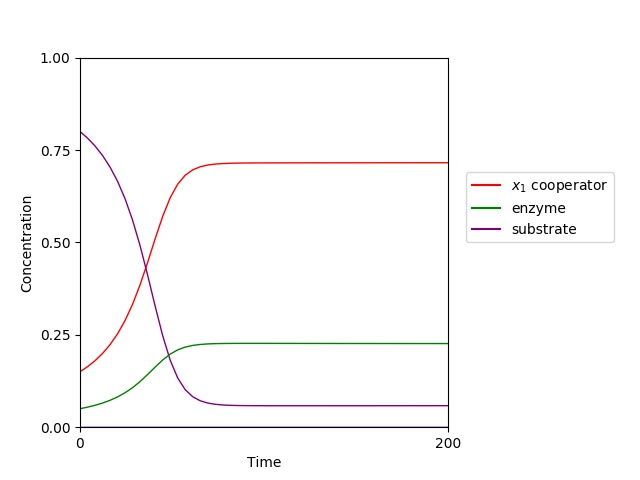
\includegraphics[width=\linewidth]{x1_1.jpeg}
\end{subfigure}
\begin{subfigure}[b]{0.45\linewidth}
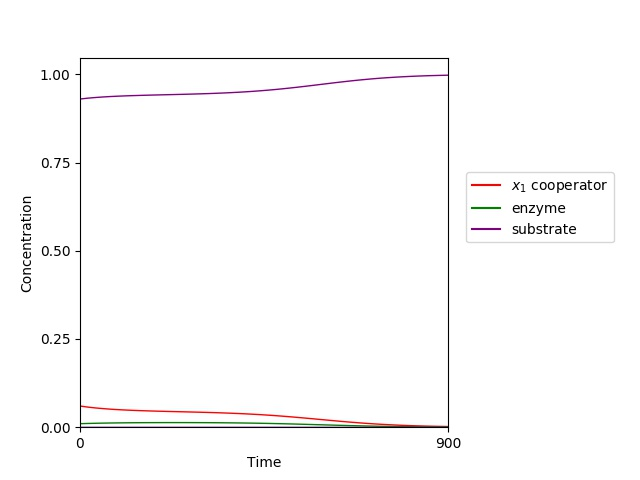
\includegraphics[width=\linewidth]{x1_2.jpeg}
\end{subfigure}
\caption{Time series for system $(\ref{s1-red})-(\ref{s4-red})$ illustrating the two locally asymptotically stable steady states for that system: The washout steady state $E_0$ (right panel) and the cooperator persistence steady state $E_1^s$ (left panel). The initial conditions used for the right panel are $s=0.93, e=0.01, x_1=0.06$;  the initial conditions for  the left panel are $s=0.8, e=0.05, x_1= 0.15.$}
\label{fig:timeser_x1}
\end{figure}

\noindent
Figure $\ref{fig:timeser_x1x3}$ illustrates that the Tragedy of the Commons occurs when there are cheaters, but no 
toxin producers or toxins, as proved in Theorem  $\ref{main00}$.

\begin{figure}[h!]
\centering
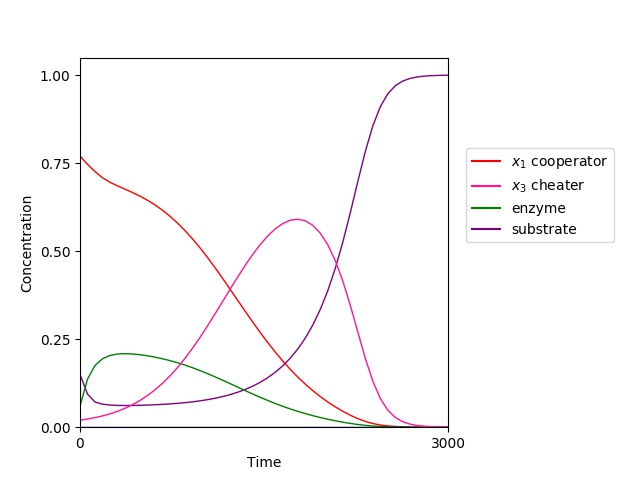
\includegraphics[width=0.45\linewidth]{x1x3_trag.jpeg}
\caption{Time series illustrating the Tragedy that occurs when cheaters are present and toxin-producing microbes are absent. The initial conditions are as follows: $s=0.15, e=0.06, x_1=0.77, x_3=0.02$, and $x_2=t=0$.}
\label{fig:timeser_x1x3}
\end{figure}

\noindent
In Figure $\ref{fig:timeser_x1x2}$ we show that a stable coexistence of cooperators and toxin 
producers is possible in the absence of cheaters, as proved in Theorem $\ref{main3}$.


\begin{figure}[h!]
\centering
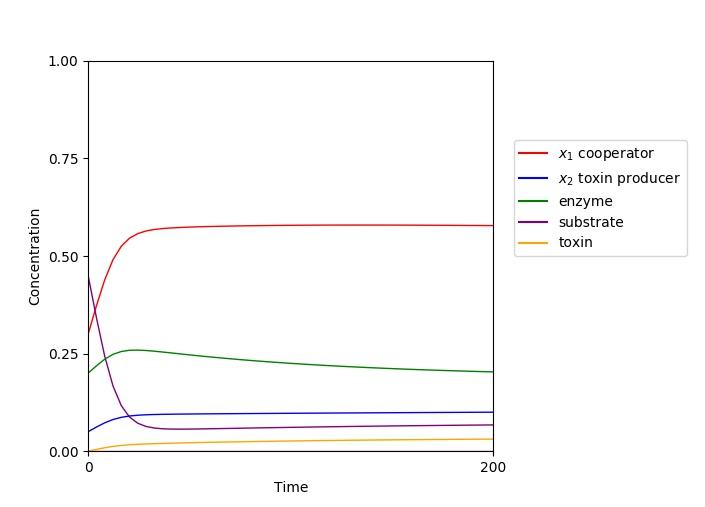
\includegraphics[width=0.45\linewidth]{x1x2.jpeg}
\caption{Time series for the system $(\ref{l1})-(\ref{l4})$ illustrating convergence to the locally stable steady state $E_{1,2}^s$. Here the initial conditions are $s=0.45, e=0.2, x_1=0.3, x_2=0.05$. }
\label{fig:timeser_x1x2}
\end{figure}


\noindent
Figure $\ref{fig:timeser_xall}$ shows two possible outcomes of the full model $(\ref{s1})-(\ref{s6})$ when cooperators, toxin producers and cheaters are present, as discussed in Theorem $\ref{main4}$. There is resistance to invasion by cheaters when $(\ref{tox})$ holds, and then the steady state 
${\cal E}_{1,2}^s$ is locally asymptotically stable. But a Tragedy occurs when 
the inequality in $(\ref{tox})$ is reversed.

\begin{figure}[h!]
\centering
\begin{subfigure}[b]{0.45\linewidth}
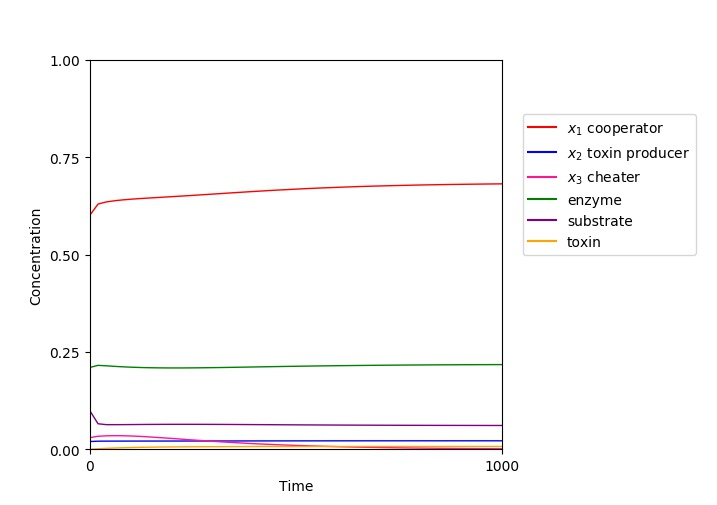
\includegraphics[width=\linewidth]{full_supp.jpeg}
\end{subfigure}
\begin{subfigure}[b]{0.45\linewidth}
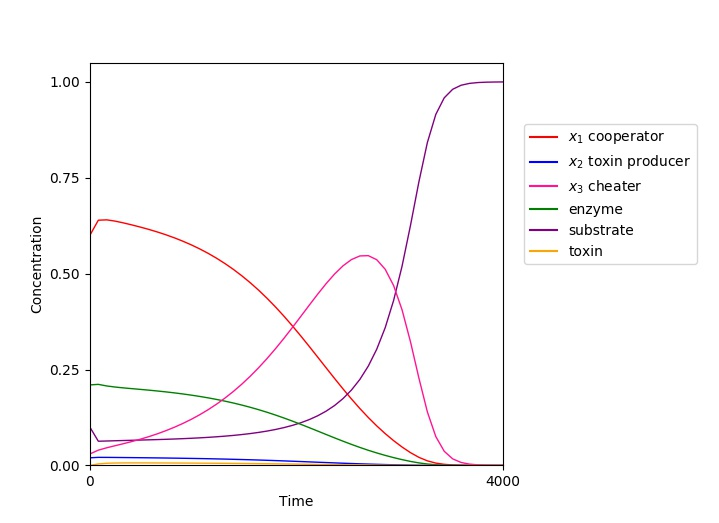
\includegraphics[width=\linewidth]{full_wash.jpeg}
\end{subfigure}
\caption{Time series for system $(\ref{s1})-(\ref{s6})$ illustrating resistance to the invasion by cheaters (left, $k_3=0.99$) or Tragedy (right, $k_3=0.3$). The initial conditions for the resistance to invasion by cheaters are $s=0.1, e=0.21, x_1= 0.6, x_2=0.02, x_3=0.03$ and the initial conditions for the Tragedy are $s=0.1, e=0.21, x_1=0.6, x_2=0.02, x_3=0.03$.}
\label{fig:timeser_xall}
\end{figure}
\FloatBarrier


\section{Conclusions}
The purpose of this paper was to investigate a division of labor model in a population consisting of cooperators who produce a public good required for growth, 
and toxin producers who produce a toxin that harms invading cheaters who do not contribute to public good or toxin production. 
We first established that a cooperator-only population can persist (Theorem $\ref{main1}$), but that it is always doomed when it is invaded by mutant cheaters (Theorem $\ref{main00}$), a phenomenon known as the Tragedy of the Commons (ToC). Our main goal was therefore to determine if the ToC can be avoided in 
the presence of toxin-producers. We first showed that the mere presence of toxin producers is not necessarily enough. Indeed, when the toxicity rate for cooperators $k_1$  exceeds the toxicity rate for cheaters $k_3$, then the entire population will still go extinct, and thus a ToC cannot be avoided (Theorem $\ref{main0}$). 
In the absences of cheaters, a mixture of cooperators and toxin producers will go extinct if the cost of cooperation $q_1$ exceeds the cost of toxin production $q_2$ (Theorem $\ref{main2}$). But a mixture of cooperators and toxin producers can coexist at a stable steady state in the absence of cheaters (Theorem $\ref{main3}$), provided that:
\begin{enumerate}
\item The cost of toxin production $q_2$ exceeds the cost of cooperation $q_1$, and 
\item The toxicity rate for the cooperators $k_1$ is sufficiently large, made precise in $(\ref{k1-large})$.
\end{enumerate}
Theorem $\ref{main3}$ was established under additional assumptions {\bf H1}, {\bf H2} and {\bf H3} imposed on the growth rate function $f(s,e)$, but these are naturally satisfied for 
commonly used growth rate functions found in the literature. We also had to make the technical assumption that $h'_1(x_{1,2}^s)$ was sufficiently small to prove Theorem $\ref{main3}$.  

Our final result (Theorem $\ref{main4}$) showed that the above mixed stable steady state of cooperators and toxin producers is resistant to invasion by cheaters, provided that the toxicity rate for the cheaters is sufficiently large; more precisely, cheaters cannot invade if
\begin{equation}\label{tox2}
k_3>\frac{q_2}{q_2-q_1}k_1.
\end{equation}
We have already mentioned above that to avoid a ToC, the toxicity rate for the cheaters $k_3$ should exceed the toxicity rate for cooperators $k_1$. Condition $(\ref{tox2})$ shows exactly how much larger $k_3$ should be; namely, $k_3$ should be larger than $q_2/(q_2-q_1)$ (a number that is strictly larger than $1$) times $k_1$. 


Our results contribute support to the idea that policing strategies may have evolved to stabilize and maintain cooperation in populations.

\newpage
\begin{thebibliography}{199}

\bibitem{xavier}	Xavier, J.B., Kim, W., Foster, K.R., A molecular mechanism that stabilizes cooperative secretions in {\it Pseudomonas aeruginosa}, Mol. Microbiol. 79:166-179,2011.

\bibitem{finkelstein}	Finkelstein, R.A., Bacterial extracellular zinc-containing metalloproteases, Microbiol. Rev. 57:823-837, 1993.

\bibitem{harrison}	Harrison, F., and Buckling, A., Cooperative production of siderophores by {\it Pseudomonas aeruginosa}, Front. Biosci. 14:4113-4126, 2009.

\bibitem{velicer2}	Velicer, G.J., Kroos, L., and Lenski, R.E., Developmental cheating in the social bacterium {\it Myxococcus xanthus}, Nature 404:598-601, 2000.
\bibitem{greig}	Greig, D., and Travisano, M., The Prisoner's Dilemma and polymorphism in yeast SUC genes, Proc. Biol. Sci. 271 Suppl. 3:S25-26, 2004.
\bibitem{ennis}	Ennis, H.L., Dao, D.N., Pukatzki, S.U., and Kessin, R.H., {\it Dictyostelium} amoebae lacking an F-box protein form spores rather than stalk in chimeras with wild type, Proc. Natl. Acad. Sci. USA 97:3292-3297, 2000.

\bibitem{hardin} Hardin, G.R., The Tragedy of the Commons, Science 162 (3859), p. 1243-1248, 1968.
\bibitem{tragedy}  Schuster, M., Foxall, E., Finch, D., Smith, H., and De Leenheer, P., 
Tragedy of the Commons in the Chemostat, PLOS ONE,  December 2017, https://doi.org/10.1371/journal.pone.0186119
(also arXiv:1705.07214 [q-bio.PE], 2017).

\bibitem{MBE} De Leenheer, P., Smith, H.L., and Schuster, M., Strong cooperation or tragedy of the commons in the chemostat, 
Mathematical Biosciences and Engineering 16, p. 139-149, 2019. doi: 10.3934/mbe.2019007 


\bibitem{hamilton} Hamilton, W.D., The genetical evolution of social behaviour I \& 2, J. Theor. Biol. 7:1-52, 1964.
\bibitem{sachs}	Sachs, J.L., Mueller, U.G., Wilcox, T.P., and Bull, J.J.,The evolution of cooperation, Quart. Rev. Biol. 79:135-160, 2004.





\bibitem{foster}	Foster, K.R., Parkinson K., and Thompson, C.R. What can microbial genetics teach sociobiology? Trends Genet. 23:74-80, 2007.
\bibitem{schuster}	Schuster, M., Sexton, D.J., Diggle, S.P., and Greenberg, E.P.,  Acyl-homoserine lactone quorum sensing: from evolution to application. Annu. Rev. Microbiol. 67:43-63, 2013.
\bibitem{ratnieks}	Ratnieks, F.L., Foster, K.R., and Wenseleers, T.,  Conflict resolution in insect societies, Annu. Rev. Entomol. 51:581-608, 2006.
\bibitem{travisano} Travisano, M., and Velicer, G.J., Strategies of microbial cheater control, Trends Microbiol. 12:72-78, 2004.
\bibitem{cheating-wikipedia}Cheating (biology), https:$//$en.wikipedia.org$/$wiki$/$Cheating$\_$(biology)
\bibitem{ratnieks2007}  Ratnieks, F.L., and Wenseleers, T., Altruism in insect societies and beyond: voluntary or enforced?, TRENDS in Ecology and Evolution 23: 45-52, 2007.
\bibitem{wenseleers} Wenseleers, T., Helantera, H., Hart, A., and Ratnieks, F.L.W., Worker reproduction and policing in insect societies: an ESS analysis, 
J. Evol. Biol. 17, 1035-1047, 2004.
\bibitem{wenseleers-bees}Wenseleers, T.,  and  Ratnieks, F.L.W., Tragedy of the commons in {\it Melipona} bees, Proc. R. Soc. Lond. B (Suppl.) 271, S310�S312, 2004.
\bibitem{wang}	Wang, M,, Schaefer, A.L., Dandekar, A.A., and Greenberg, E.P., Quorum sensing and policing of {\it Pseudomonas aeruginosa} social cheaters, PNAS 112, 2187-2191, 2015.
\bibitem{manhes} Manhes, P.,  and Velicer, G.J., Experimental evolution of selfish policing in social bacteria, PNAS 108, 8357-8362, 2011.
\bibitem{smalley} Smalley, N.E., Dingding, A., Parsek, M.R.,  Chandler, J.R., and Dandekar, A.A., 
Quorum Sensing Protects {\it Pseudomonas aeruginosa} against Cheating by Other Species in a Laboratory Coculture Model, 
Journal of Bacteriology 197, 3154-3159, 2015.

\bibitem{smith-waltman}Smith, H.L., and Waltman, P., The theory of the chemostat, Cambridge University Press, 1995.

\end{thebibliography}

\end{document}





\bibitem{SmTh} Chemostats and epidemics:competition for nutrients or host, with H. Thieme, Mathematical Bioscience and Engineering (10) December 2013, 1635-1650.

\bibitem{schuster-etal} M. Schuster, E. Foxall, D. Finch, H. Smith, and P. De Leenheer,
Tragedy of the Commons in the Chemostat,  PLOS ONE, Dec 2017,
https://doi.org/10.1371/journal.pone.0186119



\bibitem{smith-book}H.L. Smith, Monotone Dynamical Systems, American Mathematical Society, 1995.

\bibitem{smith-waltman}H.L. Smith, and P. Waltman, The theory of the chemostat, Cambridge University Press, 1995.
























